\documentclass[12pt]{comjnl}

\usepackage{amsmath}

%\copyrightyear{2009} \vol{00} \issue{0} \DOI{000}
\linespread{1.5}

\begin{document}

\title[Hashtag Segmentation of Conversational Tweets in Turkish]{Hashtag Segmentation of Conversational Tweets in Turkish, Modelling Segmentation Approach Final Report}
\author{Utku Saridede, Sevket Topuz\\
Advisor: Ass. Prof. Arzucan Ozgur\\
Co-Advisor: Arda Çelebi}
\affiliation{Degree of Bachelor of Science \\
Informational Retrival and Natural Language Processing, Department of
Computer Engineering, Bogazici University, Istanbul
Bebek 34342, TR} \email{utku.saridede@boun.edu.tr, sevket.topuz@boun.edu.tr}

\shortauthors{Hashtag Segmentation of Conversational Tweets in Turkish}

\received{07 October 2015}
\revised{12 January 2016}

\keywords{Twitter; Tweet; Tweets; Hashtag; Segmentation; Turkish; Conversational Tweets;
		Hashtag Segmentation}

\begin{abstract}	
Twitter is the latest social networking tool which affects everything related to the person.
Twitter allows its users to write at most 140 character long update, it is known off as 
``tweet''. In this research, analyzing segmentation of hashtags from tweets is our main objective. There are
several researches in English, but not that much in Turkish. Studying with the Turkish corpus is
somehow hard to study, because Turkish resources have grammer problems due to the English effect.
The usage of the hashtags differ in country to country. Having more than one word in the hashtag or lapsus calami 
prevent researchers to work properly. It is the first project in Turkey to segment tweet's hashtags in Turkish. Therefore, the results of our project is milestone in that manner. It will assist oncoming projects in the case of corpus and method needs. The other part of the project is analyzing hashtags in the way of linguistics.
Analyzed corpus will give more information about related countries. In the other words, short-term
hashtag analyses keep informed about spesific situations which influence the society. After all said
and done, we will recognize the strength of computer science on natural languages.
\end{abstract}

\maketitle
\onecolumn
\tableofcontents
\newpage

\maketitle
\section{Introduction and Motivation}
\subsection{Introduction}
\subsubsection{The Story of Hashtag}
A hashtag is a type of label or metadata letters used especially on social network and microblogging services which makes it easier for users to find messages with a specific theme or content.

The story is began with Twitter but has extended to other social media platforms as well as ``facebook''. In 2007, developer Chris Messina proposed, in a tweet, that Twitter begin grouping topics using the hash symbol. Twitter initially rejected the idea. But in October 2007, citizen journalists began using the hashtag ``\#SanDiegoFire'', at Messina’s suggestion, to tweet updates on a series of forest fires in San Diego.

\subsubsection{Decision of Hashtags}
Which characters can be defined as \#hashtag is the important part of our project.

A hashtag is defined by any string prefixed with a ``\#'', for instance, “\#freedomtomark”,
“\#shesuggest”. The string can be a single word, an acronym, or multiple words joined
together, and usually identifies the subject topic of the tweet (e.g., “\#ENG493”)
or expresses a comment about it (e.g., “\#kappamevku”).

Spaces are an absolute segmentation rule. Even if hashtag contains multiple words, they should be together. Using capital letters in between words have no meaning. (\#CahitArf). Uppercase letters will not alter search results, so searching for \#CahitArf will yield the same results as \#cahitarf.

Numbers are supported in Twiter, so as \#23NisanBayrami. However; punctuation marks, commas, periods, exclamation points, question marks and apostrophes are forbidden characters. In addition to them; asterisks, ampersands or any other special characters are also restricted ones.
There is no preset list of hashtags. Creating a brand new hashtag is simple by putting the hash before a series of words, and if it hasn't been used before, a new hashtag is invented.

\subsubsection{Origin of Implementation}
The main objective is to implement machine learning based hashtag segmentation application.

The first work was using twitter developer tools to extract tweets from Tweeter's database. In the case of hashtag extraction, there are several issues. Using large amount of raw data that 
is recieved from social media is the way of creating corpus. In the field of natural language 
processing, the essential requirements are datasets. Having realiable training and test data helps to improve
current algorithm. Because languages are flexible and few training and test data cause to 
reproduce wrong idea. It somehow clarifies why there is not enough
research in Turkish. That is because, improving datasets might help researchers to test their idea and
models in the future. 

The starting point of project is primarily based upon gathering sufficient data to avoid
backing to drawing point. That is, being blind to quantity of data causes to quit idea. Hence, the researcher should collect large amount of data, but also with well-selected contents. When the research topic comes to natural language processing, size and quantity of data is important. Extending corpus enhances current models to achieve better results.

\subsubsection{Word Segmentation}
Word segmentation means dividing a text into meaningful words. Human-beings can divide text into words with their mental process, but computer not. Word segmentation became more difficult, meanwhile not using a seperator or using more than one form for seperation. Hence, natural language processing begins after that field.

There are several methods about word segmentation. Methods will be discussed in the case of convenience with Turkish.

\subsection{Motivation}
The common problem about languages which have Latin alphabet system is deciding the word boundary. There are three types of word boundary type.

First one is using space between words. We can not use space segmentation in our project, because hashtags do not contain spaces. 
Second type is using uppercase letters at the beginning of words. It is the main seperation rule of our word segmentation. If hashtags have more than one word in it, we can check the uppercase letters to decide word boundaries. However, when it comes to real world the usage of letters in hashtags differs from the second type.
The third one is using no uppercase or using nonsense uppercases in hashtags. Because of the natural languages' aspects, datasets contain the hashtags which are the third type of boundary type.

For natural language processing, we have to determine the word's boundaries first. The method that we used tries to work on collected data to create a model that demonstrates the Turkish words' structures.

\section{State of Art}
\subsection{Related Papers and Projects}
\subsubsection{A Simple and Effective Unsupervised Word Segmentation Approach}
\subsubsection{Word Segmentation: Quick but not Dirty}
\subsubsection{A Statistical Learning Algorithm for Word Segmentation}
\subsubsection{Optimizing Chinese Word Segmentation for Machine Translation Performance}


\subsection{Improvement of Our Project}

\section{Methods}
We have tried to discourse manly with 3 methods. Hashtag segmentation can be generally defined as word boundry detection. Because of this, we
start with detection of the word boundry. There are two feature­based learning methods,
Conditional Random Fields (CRFs)(Laerty et al.,2001) and Maximum Entropy (MaxEnt).
CRFs can represent the uncommon parts of the information as elements furthermore, are great at
displaying grouping marking problems. MaxEnt is extremely compelling at learning with a high
assortment of components, without agonizing over the multifaceted nature of the model. Hidden
Markov Model is a simplistic approach for word segmentation. It helps us to built character
trigrams. It tries to catch boundary characters that are current and previous ones. Peter Norvig's
implementation can be used for word bigrams.

Manual annotation is time consuming task and it limits the amount of trainig data that can be
created. We try to achieve utilizing data to create training sets for hashtag segmentation. Synthetic
hashtags by concatenating the words in tweets can also be used for training data because word
boundries are known. To use concatenating the words in tweets as training dataset, we need to filter
non­word tokens. If tweets include non­word token in the beginnig or end of the text, it can be
removed and other words can be used as trainig data. On the other side, if a non­word token appear
in the middle of the text, the tweet is dicarded because non­word token ib the middle of the tweet
may distort the word order. The word order is important point of trainig data.

Word boundry detectiton and word segmentation is very important for Chinese words segmentation. A good research about Chinese word segmentation can be found out in Wu and Tseng's paper. A Chinese senteces do not
include delimiters to seperate words. It includes combined of a string of characters. Netural
networks and lazy learning (just-in-time learning) approaches are methods that are used in word segmentation.
Processing of the examples are collected until a clear request for information is received. When the information recieved, the databse search is completed according to amount of the distance that is most related to query.

We can use each character of training data to represent one function of learning system. Some
features should be determined and each character should be examined according to these features
to create machine learning system.

\section{Results}
We have collected the tweets from twitter. We tokenize tweets, normalize them and get 
hashtags from them. We have stored all information related to tweets. That will help us to recognize training and test data. The training data will be the part of the current data.

\begin{figure}
\centering
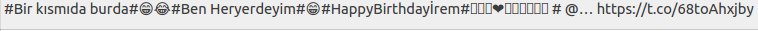
\includegraphics[width=3.5in]{tweet.png}
\caption{Tweet example.}\label{fig:Tweet}
\end{figure}

Implementing a method to get hashtags and insert them database is 
accomplished. There are two kind of table as well as "TEXTS" which contains unique tweet IDs
and tweet text.

\begin{figure}
\centering
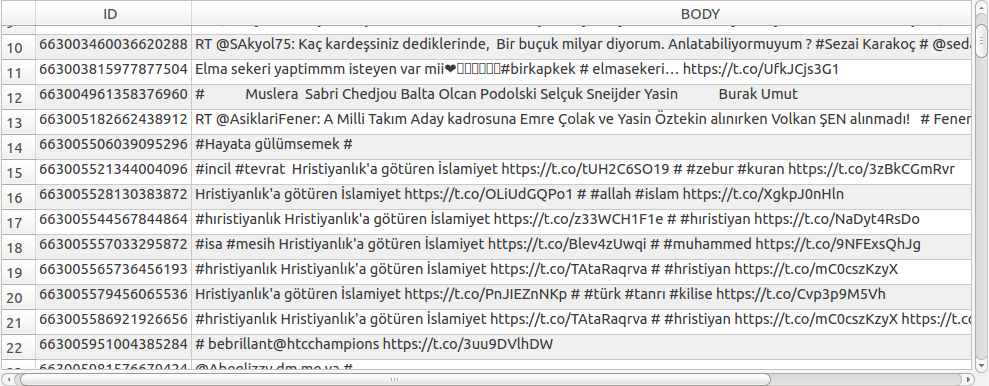
\includegraphics[width=3.5in]{text.png}
\caption{Text database table representation.}\label{fig:Tweet}
\end{figure}

The other one is "HASHTAGS" which contains tweet IDs and hashtags. Segmentation algorithm
is almost done.

\begin{figure}
\centering
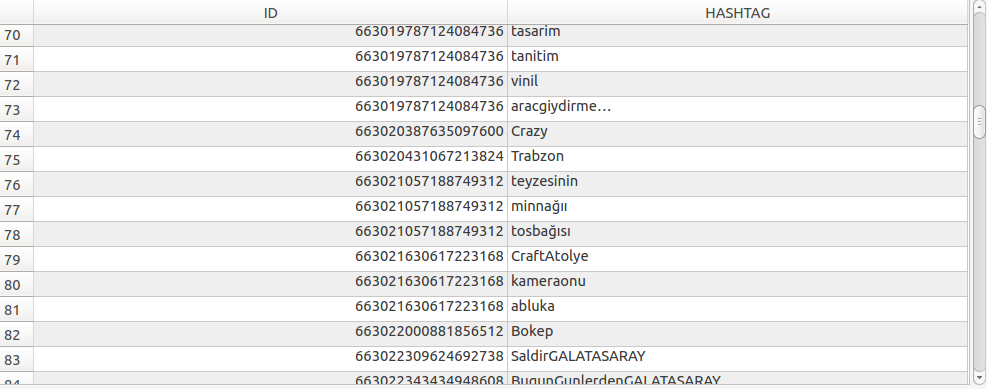
\includegraphics[width=3.5in]{hashtag.png}
\caption{Hashtag database table representation.}\label{fig:Hashtag}
\end{figure}

\section{Conclusion}
We proposed a simple and effective unsupervised
word segmentation approach. The criterion incorporates
boundary information to model words.

\section{Future Work}
We decided to improve our segmentation algorithm. Features of the words will be dicussed. Training and test
datasets will be prepared. Every word in the training data will be used to improve machine
learning power of our project. Later future works will be consulted to Prof. OZGUR.

\section{References}
- Berardi, Giacomo; Esuli, Andrea; Marcheggiani, Diego and Sebastiani, Fabrizio. Exploring the use of hashtag segmentation and text quality ranking 
Istituto di Scienza e Tecnologie dell’Informazione Consiglio Nazionale delle Ricerche 56124 Pisa, Italy

- Kan, Min-Yen, Web Page Classification

- Bansal, P., Bansal, R. and Varma V. 2015. Towards
Deep Semantic Analysis Of Hashtags.

- Berardi, G. and Esuli, A. and Marcheggiani, D. and
Sebastian, F. 2011. ISTI@TREC Microblog track
2011: exploring the use of hashtag segmentation
and text quality ranking.

- Chen, S. and Xu Y. and Chang, H. 2012. A Sim-
ple and Effective Unsupervised Word Segmentation
Approach. Proceedings of the Twenty-Fifth AAAI
Conference on Artificial Intelligence

- Xue, N. 2003. Chinese word segmentation as charac-
ter tagging.. International Journal of Computational
Linguistics and Chinese Language Processing vol-
ume 8(1)

- Wong, P and Chan, C. 1996. Chinese word segmenta-
tion based on maximum matching and word binding
force.
\nocite{*}

\bibliographystyle{compj}
\bibliography{ModellingBidders}

\section{Appendix}

\end{document}